\documentclass[12pt]{article}%

\usepackage{titlesec}
\usepackage{hyperref}
\usepackage{graphicx}
\usepackage{float}
\graphicspath{../../Images/}

\setcounter{secnumdepth}{4}
\setcounter{tocdepth}{4}

\begin{document}


\begin{titlepage}

\end{titlepage}

\tableofcontents

\section{Abstract}
Many factors play into the result of a basketball game. Basketball has many statistics commonly quoted as playing key roles in a game's outcome. Some of these stats are assists, turnovers, rebounds and shooting percentage. This study attempts to develop a machine learning classification algorithm to predict the eventual winner of a game given the known per-game averages of various metrics for the two teams.

\section{Introduction}
Predicting the outcome of a sports match is a dream of gamblers the world over for. Even just a slightly successful model would be immensely profitable for a gambler. With thousands of games a year, a slight statistical advantage would lead a bettor to approach the expected value of their bets and produce consistent gains year to year.
\newline\newline
In basketball, the key is to finish the game with the most points. A team can either score points by making a two-point shot, three-point shot or various one-point "free throws". There are many different statistics typically tracked by fans and teams alike to attempt to glean a better understanding of the teams and players and their performances. Several commonly tracked stats are turnovers (losing possession of the ball to other team), assists (a key pass leading to points being scored), rebounds (securing a ball after a missed shot for another possession) and shooting percentages (percentage of shots made). Dean Oliver famously developed his model for determining how a team wins a game, called the "Four Factors of Basketball Success".\textsuperscript{1} The four factors are shooting, turnovers, rebounding and free throws. The four factors are tracked for both offense and defense so in essence it is really eight factors.
\newline\newline
In this paper, a classification algorithm is run on data for NBA (National Basketball Association) seasons from 2010 to 2019 to determine if there is potential for predicting the outcomes of games. Several different classifiers and input feature sets are used on the dataset.
\newline\newline
Due to the potential for the size of this problem if extrapolating the data to more seasons, more leagues (college, foreign, gendered) the data would grow into the realm of "Big Data". Big Data is traditionally described as following the 5V model. The five Vs are volume, velocity, variety, veracity and value.
\newline\newline
With over 100 leagues across the globe, tens of teams per league, and tens of games per season, there are the potential for millions of games a year. Then, if we use past years for data as well, then there are tens of millions of games to collect data on. Any given day, there can be many games occuring with realtime results for team performances and stats. Each game can have different types of data, from numbers for the stats, to geographic data for game location, date and time data, strings for referee names and more. In the nba, there have several relational datasets with team ids, game ids, referee ids and more being used as keys to relate the different datasets. Since a lot of data is put online for fans to check on scores, there is the potential for incorrect data either by improperly posting data online, improper data collection (different teams may record a different stat for a play such as if an assist occured or not), or corrupted data downloads. It is important to make sure all the data is accurate. Of course, if everything works and a classifier can "beat the house" in Vegas, then there is huge potential for profit.


\section{Setup}
The development of a big data solution to predicting basketball games can be broken down into several key steps. The following list will discuss the different steps and how they were achieved in the big data lifecycle.

\begin{enumerate}
\item Business Case Evaluation - It is important before tackling such a large task, to determine if there is a business case for the problem. As previously described, there is a clear business case here as a successful classifier would bring in considerable revenue.
\item Data Identification - The datasets needed are per game statistics for each game to train the classifiers and seasonal per team game averaged statistics for predicting game outcomes.
\item Data Acquisition and Filtering - The data is gathered by both webscraping and calling the official NBA.com API to pull the data off their servers. A lot of data is not necessary for this build, and is filtered out in the acquisition step. This mainly includes various statistics that were not tracked (such as game time and game location).
\item Data Extraction - The data is then transformed from the json string objects returned from the acquisition step into a dataframe object to properly setup the data to be used later.
\item Data Validation and Cleansing - The data is checked for any inaccuracies (for example throwing out preseason and postseason games).
\item Data Aggregation and Representation - The data is then setup in two different dataframes object. There is a team dataframe object that tracks the statistics for each team in each season. The key for the dataframe is a season and team id to uniquely define each observation. The per game statistics are colllected into a large game dataframe object that uses the game id and a flag for home team to uniquely define each observation.

\end{enumerate}

The data analysis, data visualization and utilization of analysis of results are defined further in the report.

\section{Methodology}
The first step in the process was identifying and collecting the data. The official NBA website has several diferent URLs to visit to look at statistics. For the game statistics, there were three different addresses used to collect data. First, a loop over each year and each day was used to get the scores for that date by calling the NBA website's API to collect the game ids for each game that occurred that day. Once all the game ids were collected, a loop over the game ids was used to collect the data. Each game id has several different addresses for the various types of statistics they keep. There is traditional game statistics, summary game statistics and advanced game statistics for example. The NBA API was called once again to pull the various stats of interest that will be used to build the classifier. The same concept was repeated for the team stats, but here there is no need to loop over days to get any game ids because each year has only one team stats webpage. The scraping code can be fonud in the apppendix. The finished data acquisition and preprocessing was subsequently saved to comma separated files.
\newline\newline
There classifier was built to run on two different sets of data. The first is the raw statistical data and the second is a four factors data setup. The raw statistical data did not require additional preprocessing but the four factor did have to be setup. The four factors and shooting, free throws, rebounding and turnovers. Only rebounding has a different calculationg for offense and defense. Otherwise, the defensive metric is just the stats of the opposing teams offense. There equations are as follows:
\begin{equation} Shooting = (FGM + 0.5 * 3PM) / FGA \end{equation}
\begin{equation} Turnovers = TOV / (FGA + 0.44 * FTA +TOV) \end{equation}
\begin{equation} Free Throws = FTM / FGA\end{equation}
\begin{equation} Rebounding_{offense} = ORB / (ORB + OpposingDRB) \end{equation}
\begin{equation} Rebounding_{defense} = DRB / (OpposingORB + DRB) \end{equation}

\begin{itemize}
\item FGM - Field Goals Made
\item 3PM - Three Pointers Made
\item FGA - Field Goals Attempted
\item TOV - Turnovers
\item FTA - Free Throws Attempted
\item FTM - Free Throws Made
\item ORB - Offensive Rebounds
\item DRB - Defensive Rebounds
\end{itemize}

A new dataframe for the four factors was created based on all the input data. The classifier was then setup to run on either the four factor or raw statistical data to try both methods to create the best possible classifier.
\newline\newline
Several different classifiers were tested to determine which may perform the best. The classification accuracy and the runtimes for each classifer were tracked to help decide the optimal classification method. The classification methods used were a random forest, support vector machine with a radial basis function kernel and a logistic classifier. These were chosen as they have significantly different designs for classfication and all would work well on the many-input data.
\newline\newline
The training and testing setup is not as cut-and-dry as typical classifiers as the training data and testing are different. First, the games were randomly shuffled and split into training (75\% of data) and testing (25\% of data) datasets. The classifiers were trained on the per game statistics to learn who would win a game. The input features were the home team's stats minus the away team's stats and the target class was whether the home team won or not. Therefore, the classifier is learning whether a home team would win given the input statitistics. If a home team had 15 personal fouls and the away team had 17 then the input feature for personal fouls would be negative 2. After training the data, the classifier was ran on the testing dataset to see if it would generalize well. However, this is not the true testing dataset, since we do not want to predict who would win a game based on statistics after a game had already finished. Instead, the testing dataset is then to use the same testing game ids, but then use the team's per game averages to predict if the home team would win. The game ids were gathered and then the home team and away teams per game averages were subtracted and used as the input features. For example, if the home team averages 14.7 personal fouls per game and the away team averages 10.6 personal fouls then the input for personal fouls would be 4.1. The score for this classification was called prediction accuracy. The final accuracy tracked was called control accuracy. The control accuracy was the accuracy of using a naive classification decision of simply choosing the team with the better record to win each game.
\newline\newline
The classification was trained and tested on each season from 2010 through 2018 and the performances are shown in boxplots.
\section{Results}
The first thing checked when runnning the classifiers was the correlation between input features and the target variable of who won. Figures 1 and 2 contain the plots made for correlation of the raw data and the four factors data.


\begin{figure}[H]
\caption{Correlation Matrix for Raw Statistics}
\centering
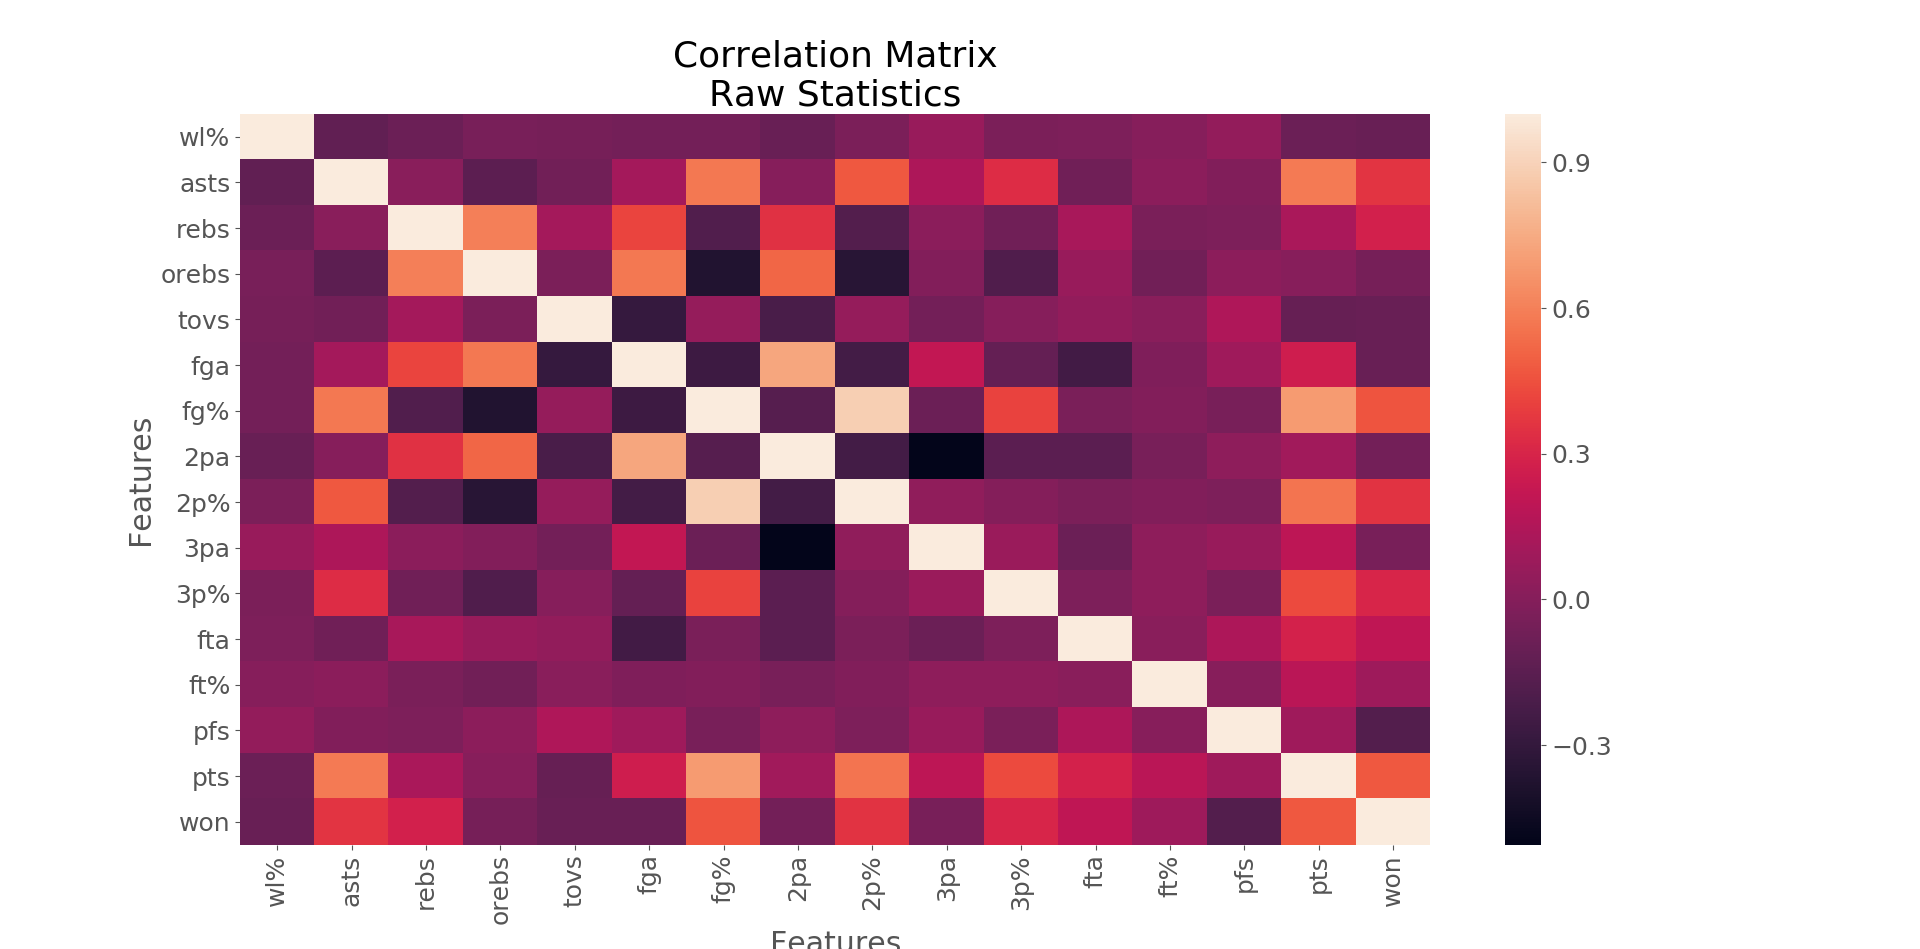
\includegraphics[width=\textwidth]{"C:/Users/paul.abers/Documents/test/588/Basketball/Images/raw_corr.png"}
\end{figure}

\begin{figure}[H]
\caption{Correlation Matrix for Four Factor Statistics}
\centering
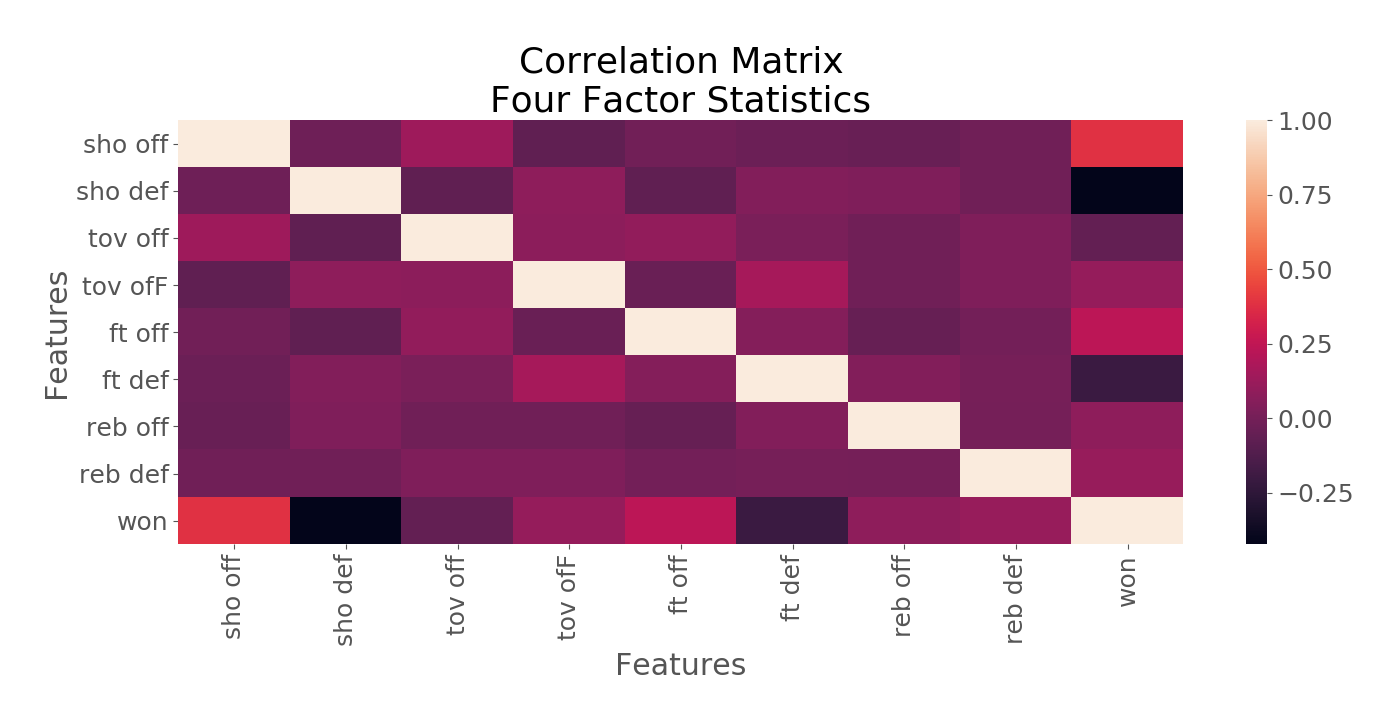
\includegraphics[width=\textwidth]{"C:/Users/paul.abers/Documents/test/588/Basketball/Images/ff_corr.png"}
\end{figure}

Some interesting aspects about the data can be gleaned from the correlation matrices. In figure 1, we can see that points, field goal percentage, assists, and rebounds have the strongest correlation with winning. This is similar to what the four factors claim (minus free throws). Another interesting note is that two pointers attempted and offensive rebounds are highly correlated. In figure 2, we see that offesnive shooting has the strongest correlation with winning. There appears to be minimal correlation between any of the input features, which is good as they each appear to present new information.
\newline\newline
Next, the classifiers were set up and run on the two datasets. The four classification accuracies (train, test, prediction and control) are plotted for the three differeent classifiers on the two datasets in figures 3 and 4. Their runtimes are displayed in table 1.

\begin{figure}[H]
\caption{Performance Accuracy for Raw Statistics}
\centering
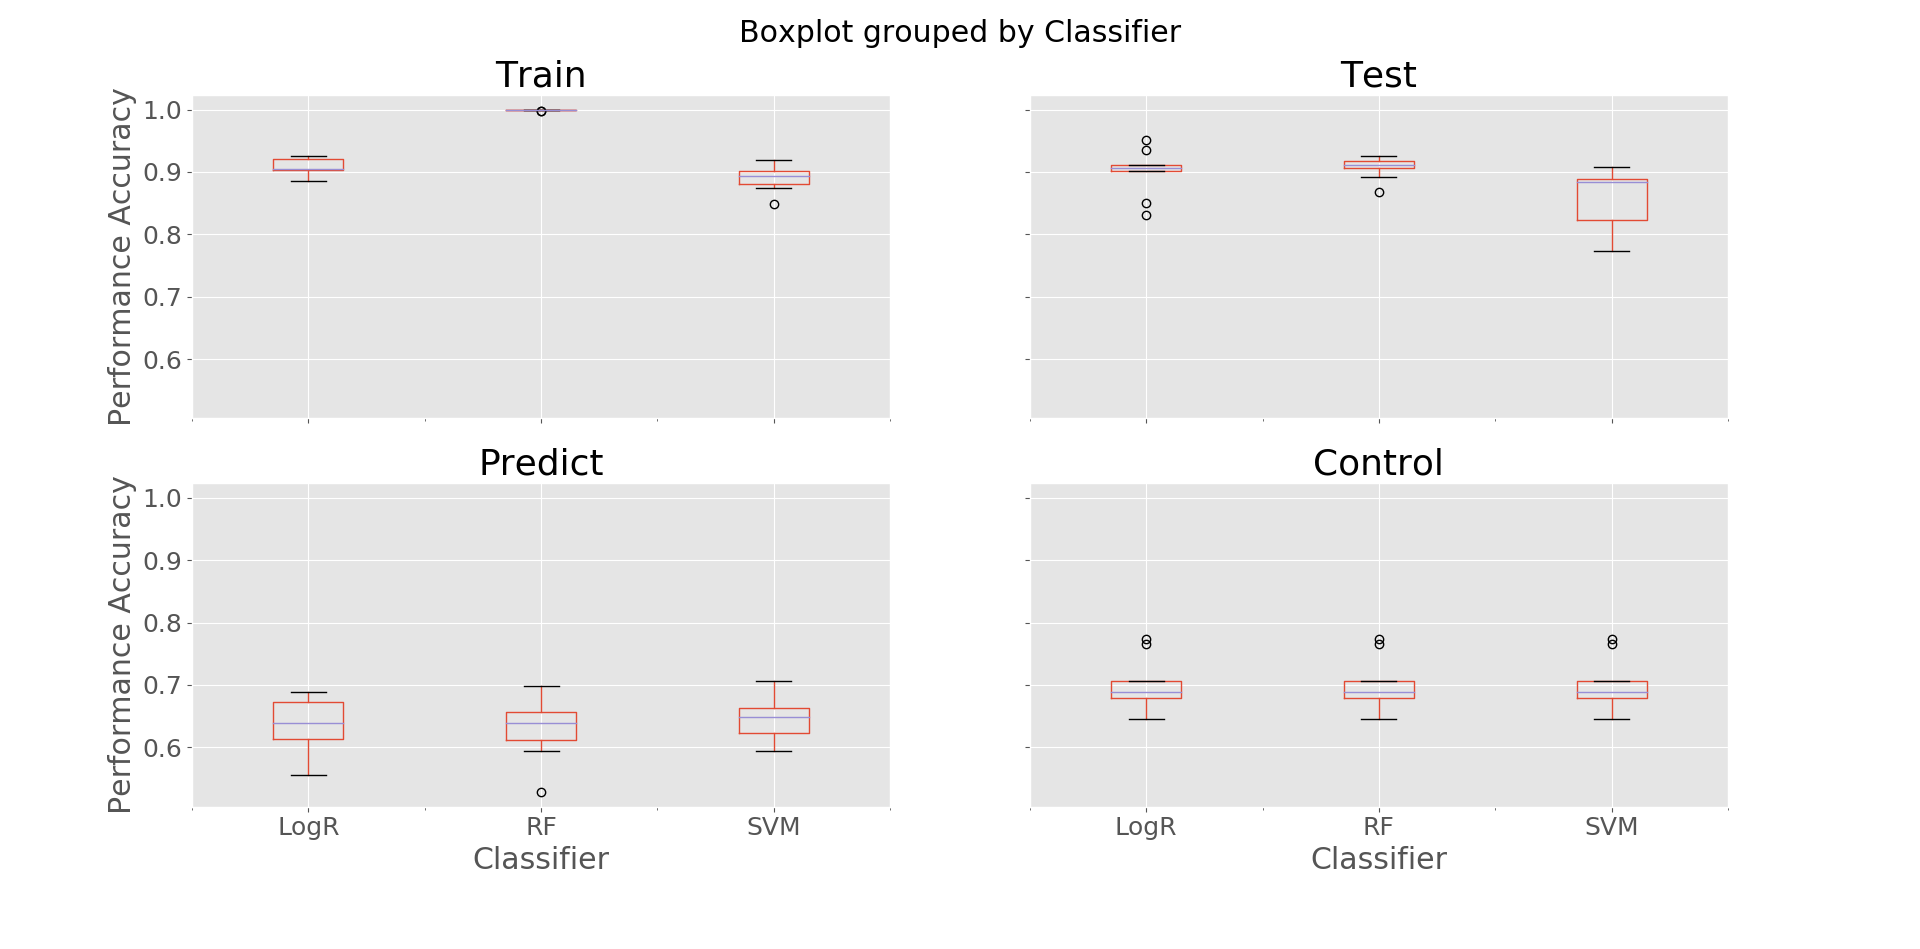
\includegraphics[width=\textwidth]{"C:/Users/paul.abers/Documents/test/588/Basketball/Images/raw_acc.png"}
\end{figure}

\begin{figure}[H]
\caption{Performance Accuracy for Four Factor Statistics}
\centering
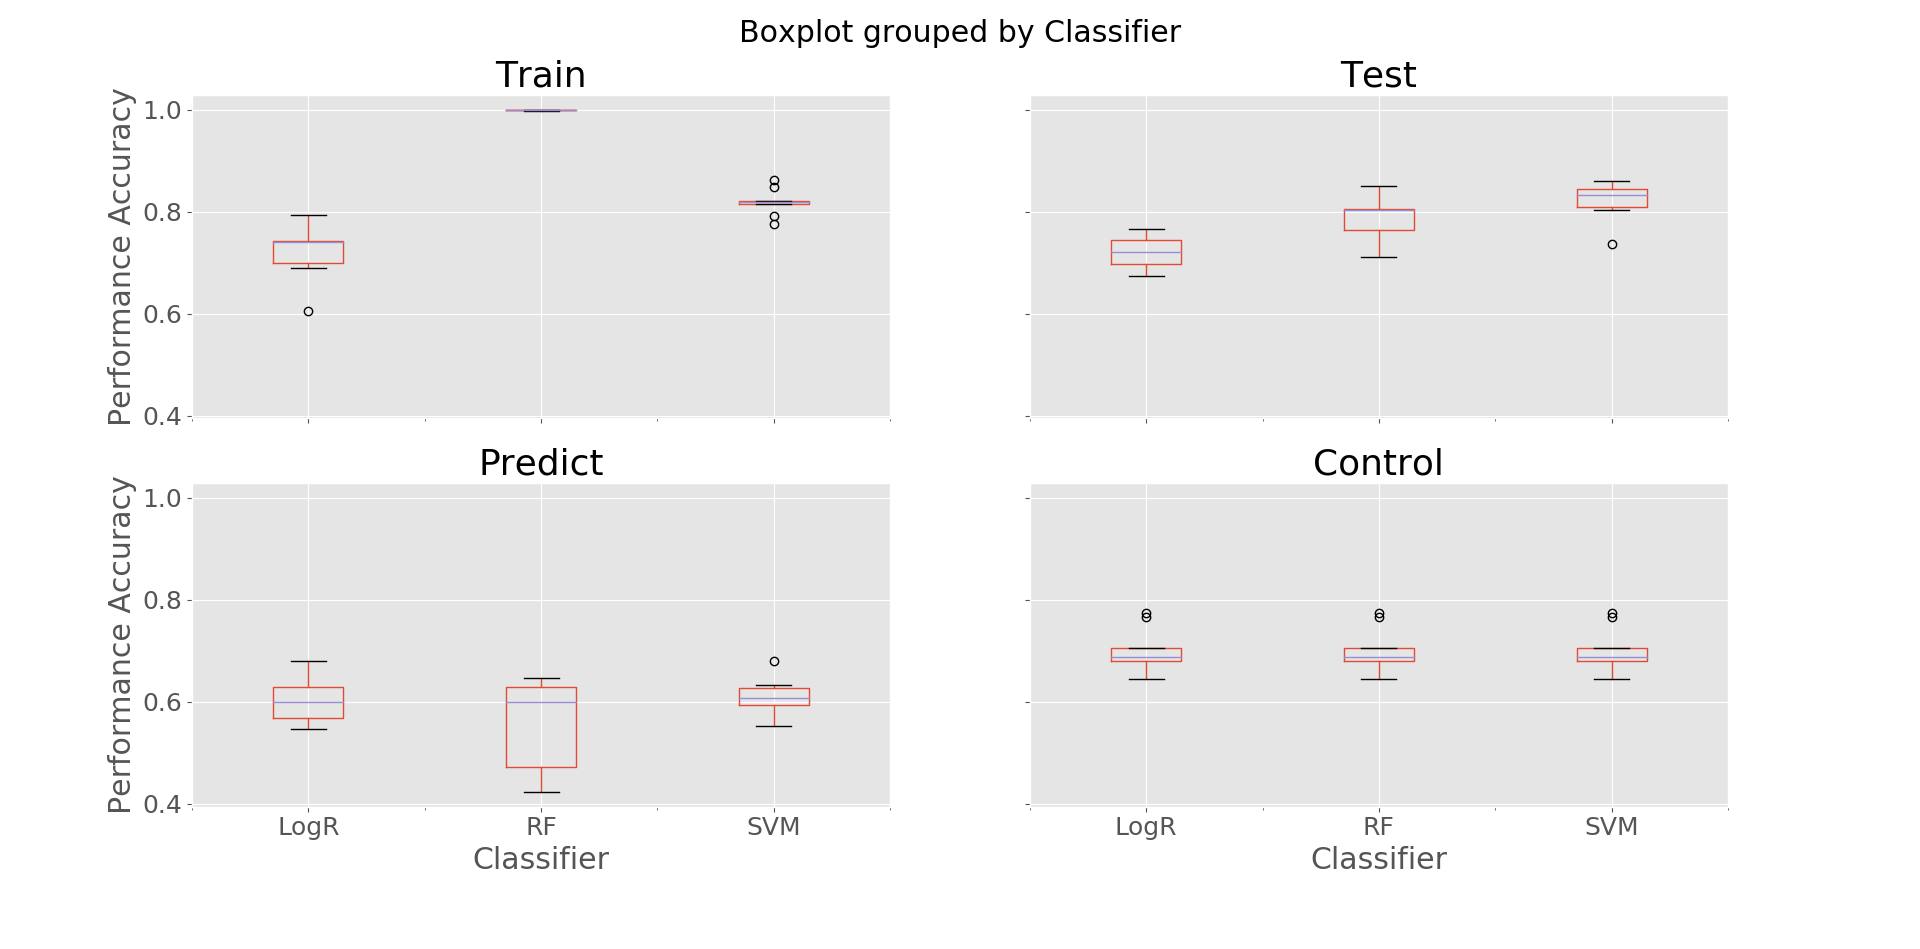
\includegraphics[width=\textwidth]{"C:/Users/paul.abers/Documents/test/588/Basketball/Images/ff_acc.png"}
\end{figure}

\begin{table}[H]
\caption{Average runtimes for classification of each season}
\begin{center}
\begin{tabular}{ || c || c | c|| }
  \hline
  Classifier & Raw Statistics & Four Factor \\ [0.5 ex]
  \hline\hline
  Logistic Regression & 0.80s & 5.12s \\
  \hline
  Random Forest & 1.12s & 4.43s \\
  \hline
  Support Vector Machine & 0.82s & 4.96s \\
  \hline
\end{tabular}
\end{center}
\end{table}


Due to the lack of improvement of the classifiers versus the control classification accuracy, principal component analysis (PCA) was also attempted on the raw dataset to determine if that would improve the performance. However, its performance was no statistically different from the previous methods.

\section{Discussion}
Based on the results from the three different classifiers on the three different datasets (raw, four factor and pca), it appears that the design and implementation of the algorithm was unsuccessful in providing any use case for a business. The classifier does perform much better than simple chance on predicting whether a home team would win a game or not, but using a simple predictor based on records achieves just as strong of a performance. The average yearly performance of the predictions and the control are within agreement given their standard deviations. Thus, while the classifiers are working somewhat and can predict which team will win based purely on several statistics (assists, rebounds, et.c.), it is just not usable for any business situation.
\newline\newline
The problem with this design and implementation resides in several different situations. The biggest issue in my opinion is that no thought is given to the important day to day differences of games. These can include key players being out (whether due to injury, sickness or rest), the second game of a back to back (teams on the second day of a back to back tend to be tired and perform at lower levels) or long road trips (similar to back to backs). A possible method to alleviate these stressors is to use active player's per game averages and sum them to create the team's per game averages. Features could also be added to flag if a team is on a back to back and a count for the away team's current road trip length. It is hard to say if these changes would drastically improve the learner but it would at least remove these elements as being possible sources of error.
\newline\newline
Another key issue in trying to beat the naive record classifier is that the quality of a team's statistics and their record are typically tightly coupled. Teams that win games tend to have more assists, less turnovers, more rebounds et.c. so you would expect these stats to predict similar to their record. In the end, it appears that a record is in essence a summary statistic for the rest of these stats and the important separation lies elsewhere (possibly in the back to back or road trip features). Also, upsets are inevitable in sports and no matter how obvious an answer on paper may seem, the final outcome always can differ from expectations. The ability of an underdog to win any given day is what makes sports so intriguing and exciting for so many people. There are a numbe of famous cinderella stories and a classifier will always struggle to find these cases as their odds are so miniscule. For example, in 2016 Leicester City (an English soccer team) overcame their 5000-to-1 odds to win the English Premier League. A classifier would never choose this as the expected outcome and so could never capture this data point.

\section{Conclusion}
In the end a classifier was proven to work and performed well enough on predicting the winner of a game based solely on their peripheral statistics but was unable to outperform a simplistic model based on team's records. The results section show the performances of the various models on the datasets created. As mentioned in the discussion, there is still some areas for possible improvement but that would require significantly more time to determine the efficacy of those additional methods. Predicting sporting events will always have their struggles due to the nature of the underdog, but it is still possible that there is untracked key features that could elicit a strong enough performance to allow a business case for using the classifer. It is only necessary to beat the odds by a small margin consistently to make the venture profitable. As the law of large numbers says that the mean value of randomly sampling a distribution approaches the expected value.\textsuperscript{2}

\section{References}
\begin{enumerate}
\item [1] Basketball Reference "Four Factors". \\
  https://www.basketball-reference.com/about/factors.html
\item [2] Routledge, Richard. "Law of Large Numbers". Brittanica Oct 12, 2016, https://www.britannica.com/science/law-of-large-numbers
\end{enumerate}

\section{Appendix: Source Code Files}
\begin{itemize}
  \item scrape\_game\_stats.py - Makes put and get requests with the NBA website for specific year to collect various statistics for each game that occurred in the various years specified. Saves the output to a comma separated file to allow easy reading in of the data for analysis.

  \item scrape\_team\_stats.py - Makes put and get requests with the NBA website for specific year to collect various statistics for each team's per game averages that occurred in the various years specified. Saves the output to a comma separated file to allow easy reading in of the data for analysis.

  \item analysis.py - Performs all the analysis on the collected data. Reads in the data, creates the input feature and target datasets and performs classification on the data. Has two main functions to call, either main() for classifying on raw statistics and main\_ff() to classify on the four factor statistics. Creates plots for the correlation matrix and the performance of the classifiers and prints the average runtimes to stdout.

\end{itemize}

\end{document}

%%% Local Variables:
%%% mode: latex
%%% TeX-master: t
%%% End:
